\documentclass[../main]{subfiles}
\begin{document}

\newpage
\chapter*{図表}
\addcontentsline{toc}{chapter}{図表}

% fig and table settings
\renewcommand{\figurename}{Fig. } % 図 -> Fig.
\renewcommand{\tablename}{Table } % 図 -> Fig.


\vspace*{\stretch{1}}
\begin{figure}[H]
  \centering
  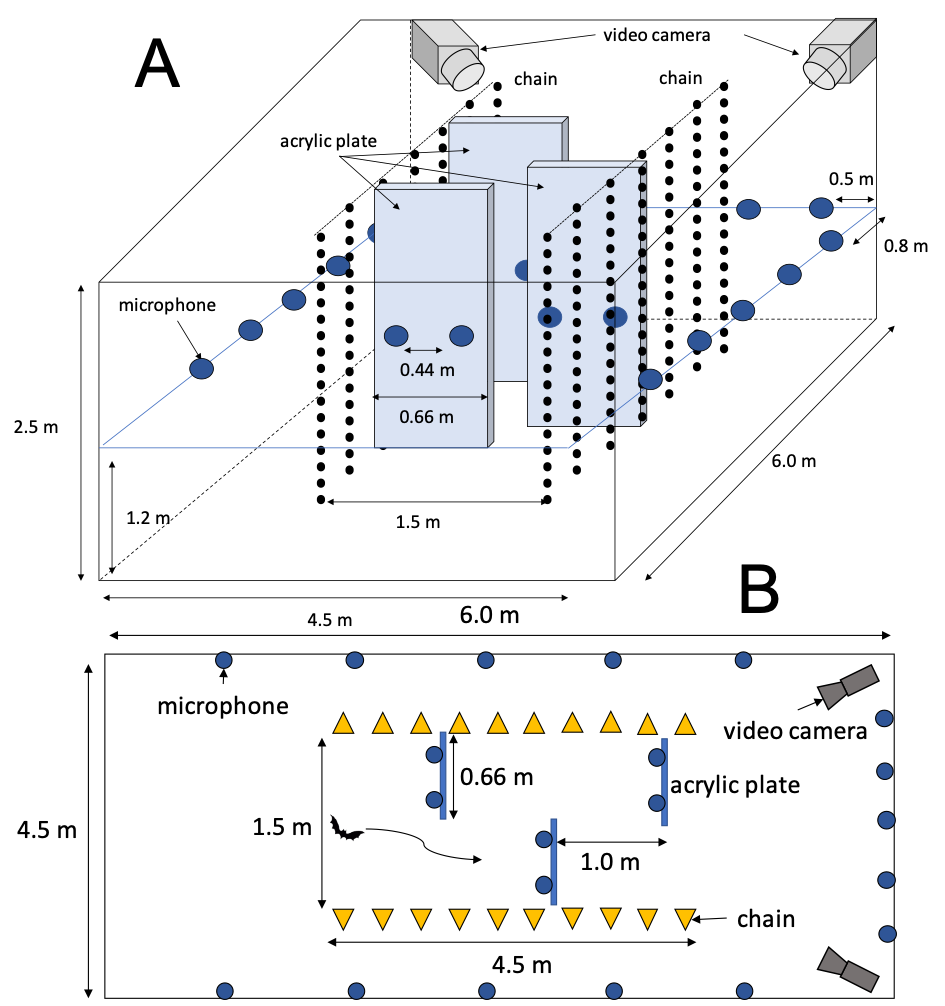
\includegraphics[width=12cm]{figures/top_view_measure.png}
  \caption{
    Top view of measurement system of flight trajectory,
    pulse direction.
  }\label{fig:top_view_measure}
\end{figure}
\vspace{\stretch{1}}

\newpage
\vspace*{\stretch{1}}
\begin{figure}[H]
  \centering
  \vfill
  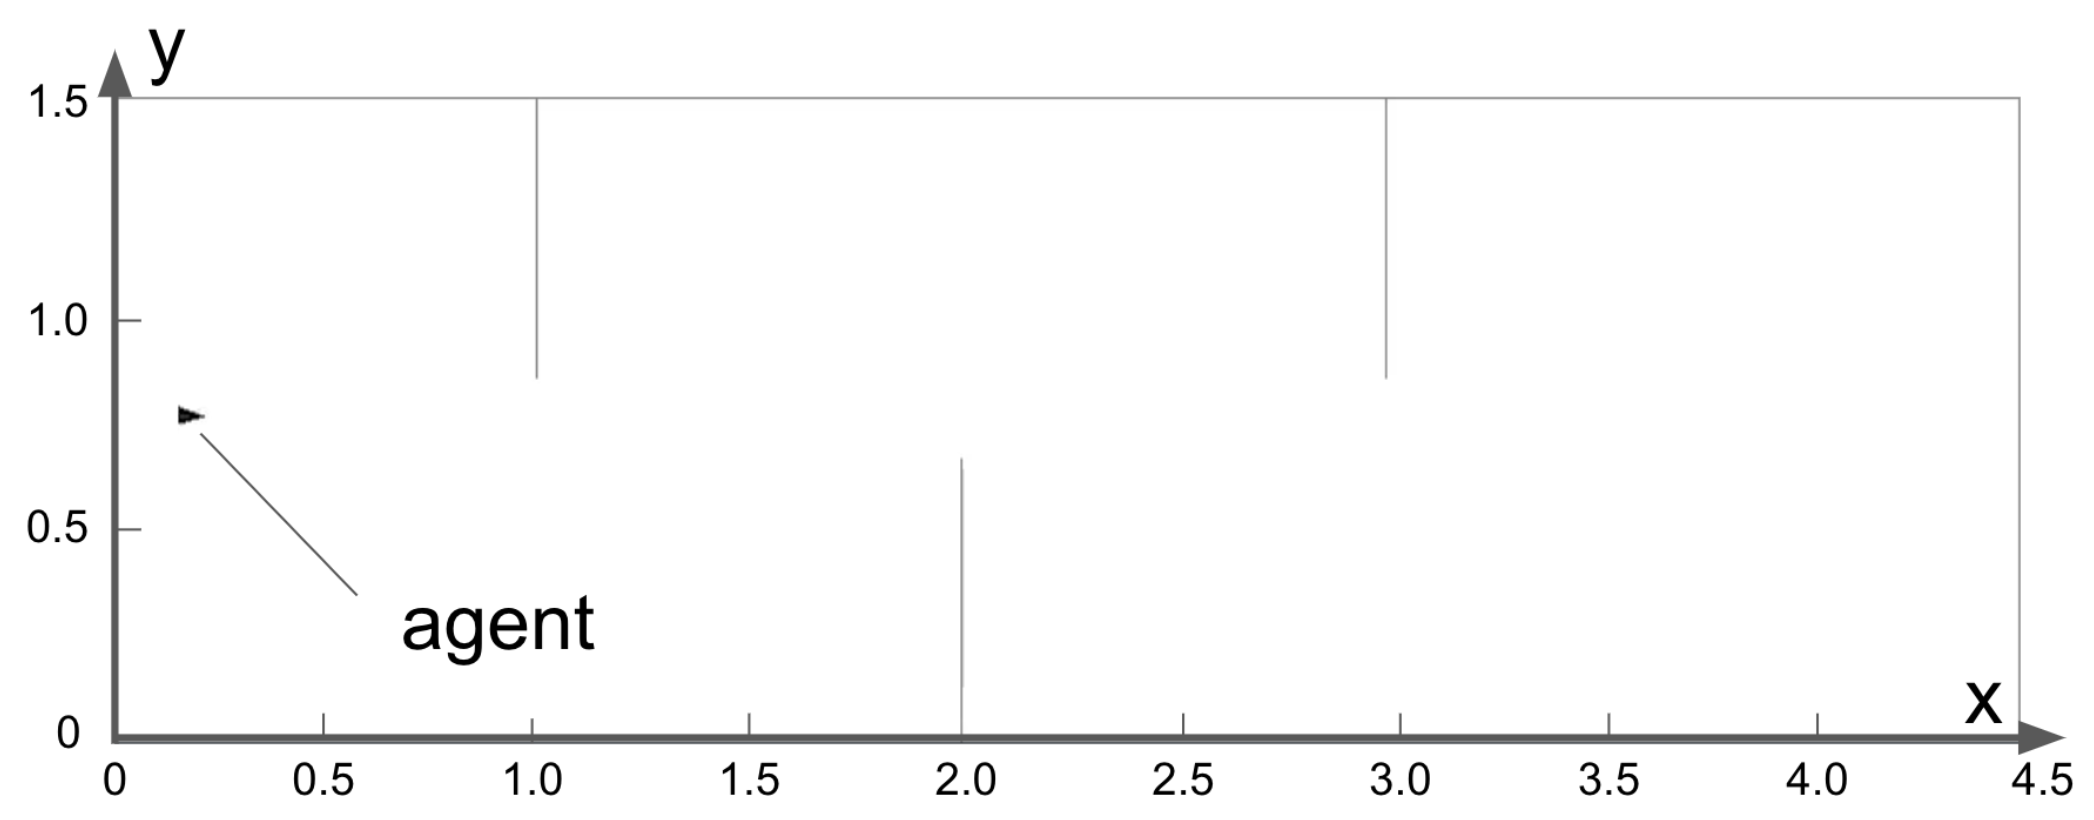
\includegraphics[width=14cm]{figures/simulation_field.png}
  \caption{
    Simulation field.
    Start point for agent is (0.2±0.05, 0.7±0.05).
    The gray lines are obstacles.
  }\label{fig:simulation_field}
\end{figure}
\vspace{\stretch{1}}


\newpage
\vspace*{\stretch{1}}
\begin{table}[H]
  \caption{Agent's actions}\label{tab:agent_actions}
  \centering
    \begin{tabular}{c|c|c}
      Action & Description & Value range \\ \hline
      $\Delta\theta_t$ & Angle to change direction & $[-\pi/4, \pi/4]$ \\
      $p^{emit}_t$ & Probability to emit pulse & $[0.3, 0.8]$ \\
      $\phi_t$ & Direction to emit pulse & $[-\pi/4, \pi/4]$ \\
    \end{tabular}
\end{table}
\vspace{\stretch{1}}


\newpage
\vspace*{\stretch{1}}
\begin{figure}[H]
  \centering
  \vfill
  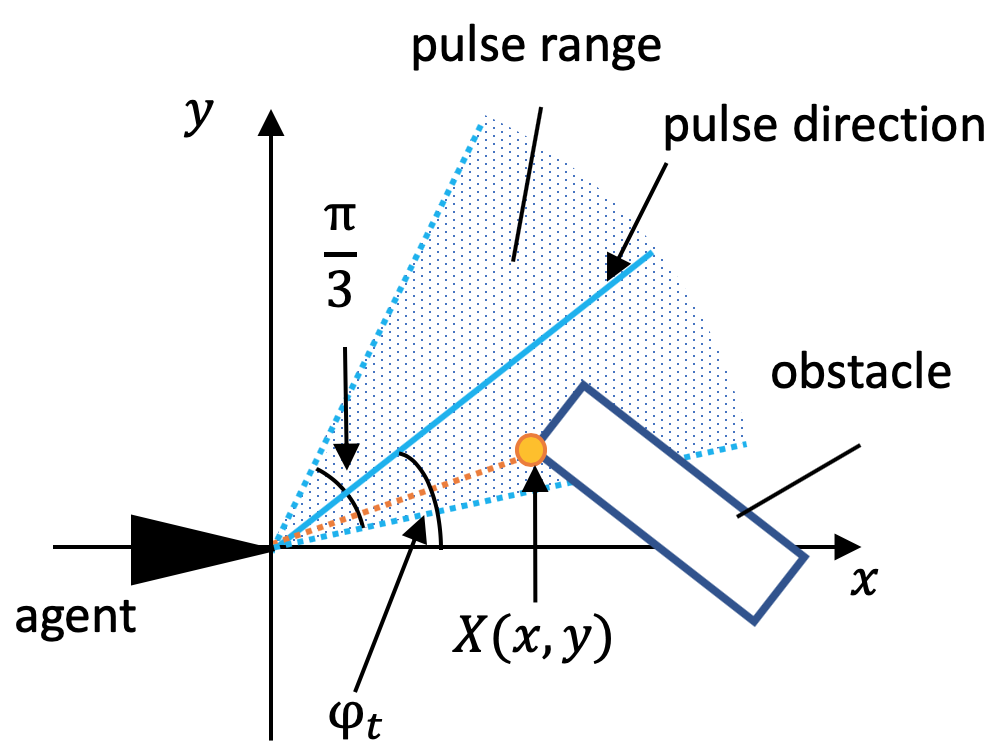
\includegraphics[width=10cm]{figures/pulse_simulation.png}
  \caption{
    Pulse simulation algorithm. Agent obtains X,
    the nearest point of the obstacle in pulse range from itself.
  }\label{fig:pulse_simulation}
\end{figure}
\vspace{\stretch{1}}


\newpage
\vspace*{\stretch{1}}
\begin{table}[H]
  \caption{The values of reward function weights.}
  \label{tab:reward_weights}
  \centering
    \begin{tabular}{c|c|c}
      Weight & Value      & Description \\ \hline
      $w_1$  & $1$        & moving reward\\
      $w_2$  & $-10$      & punishment for chaging direction\\
      $w_3$  & $-10^{-3}$ & punishment for emitting pulse \\
      $w_4$  & $-10^{-3}$ & punishment for pulse direction\\
      $w_5$  & $-10^2$    & punishment for bumping\\
    \end{tabular}
\end{table}
\vspace{\stretch{1}}



\newpage
\vspace*{\stretch{1}}
\begin{figure}[H]
  \centering
  \vfill
  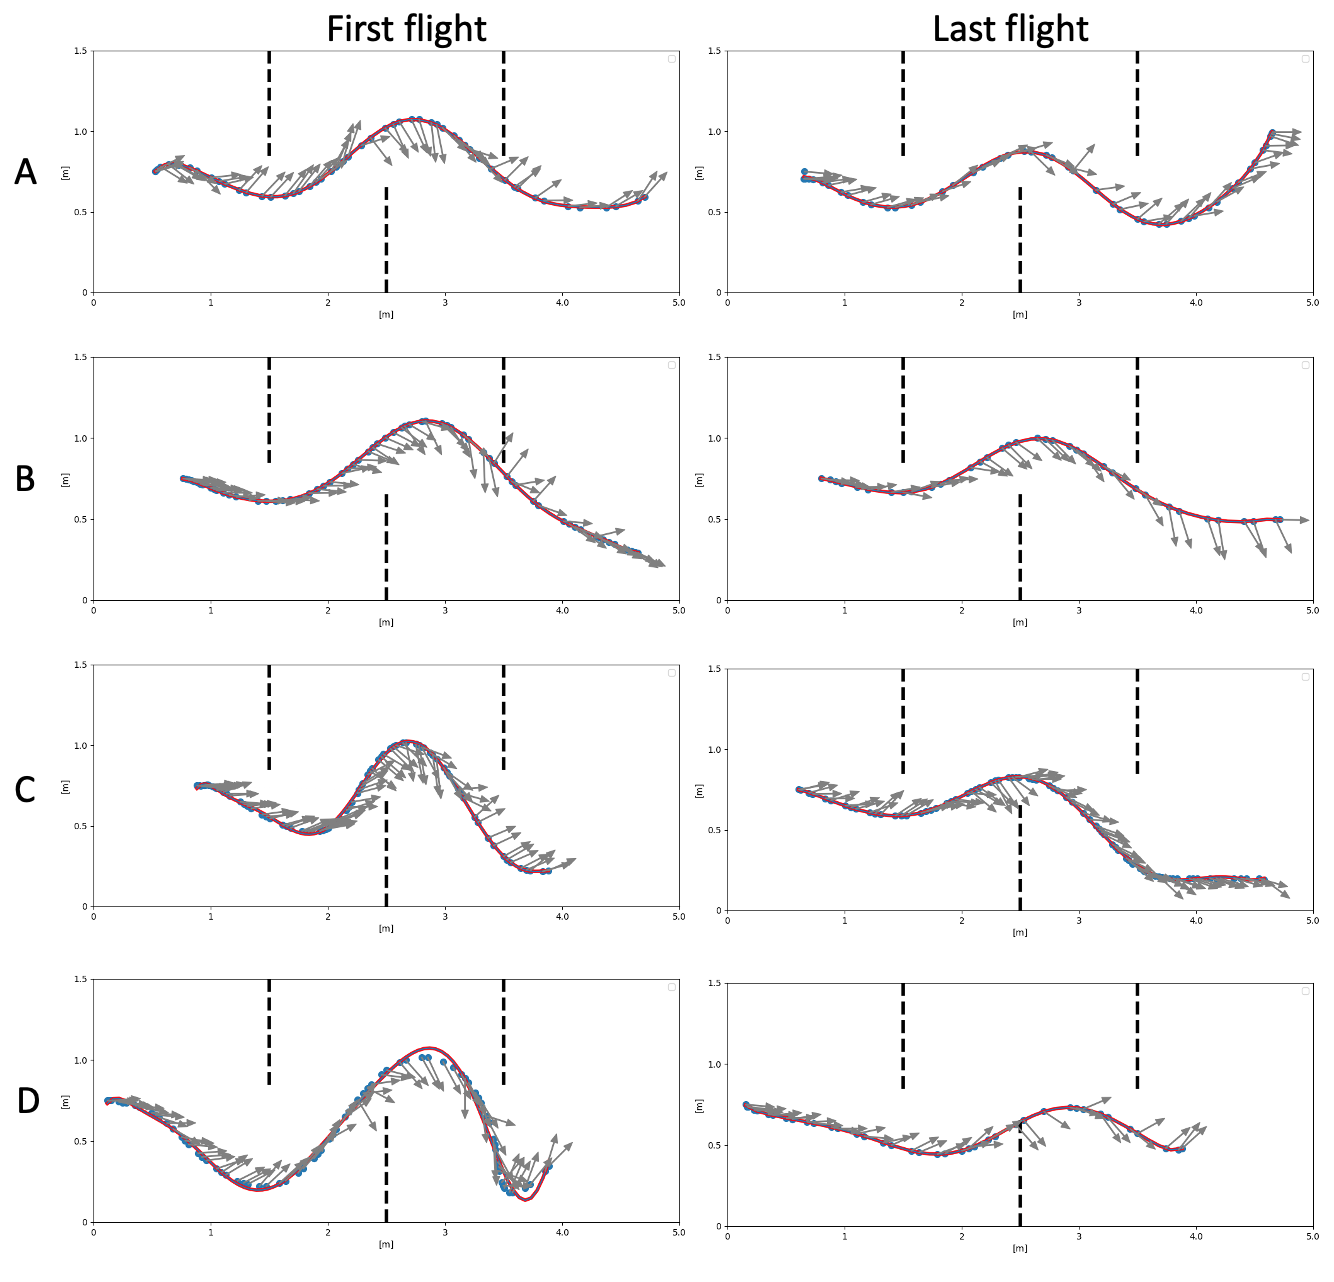
\includegraphics[width=14cm]{figures/bat_trajectories.png}
  \caption{
    Comparison between the first and last flight of the bat.
  }\label{fig:bat_trajectories}
\end{figure}
\vspace{\stretch{1}}

\newpage
\vspace*{\stretch{1}}
\begin{figure}[H]
  \centering
  \vfill
  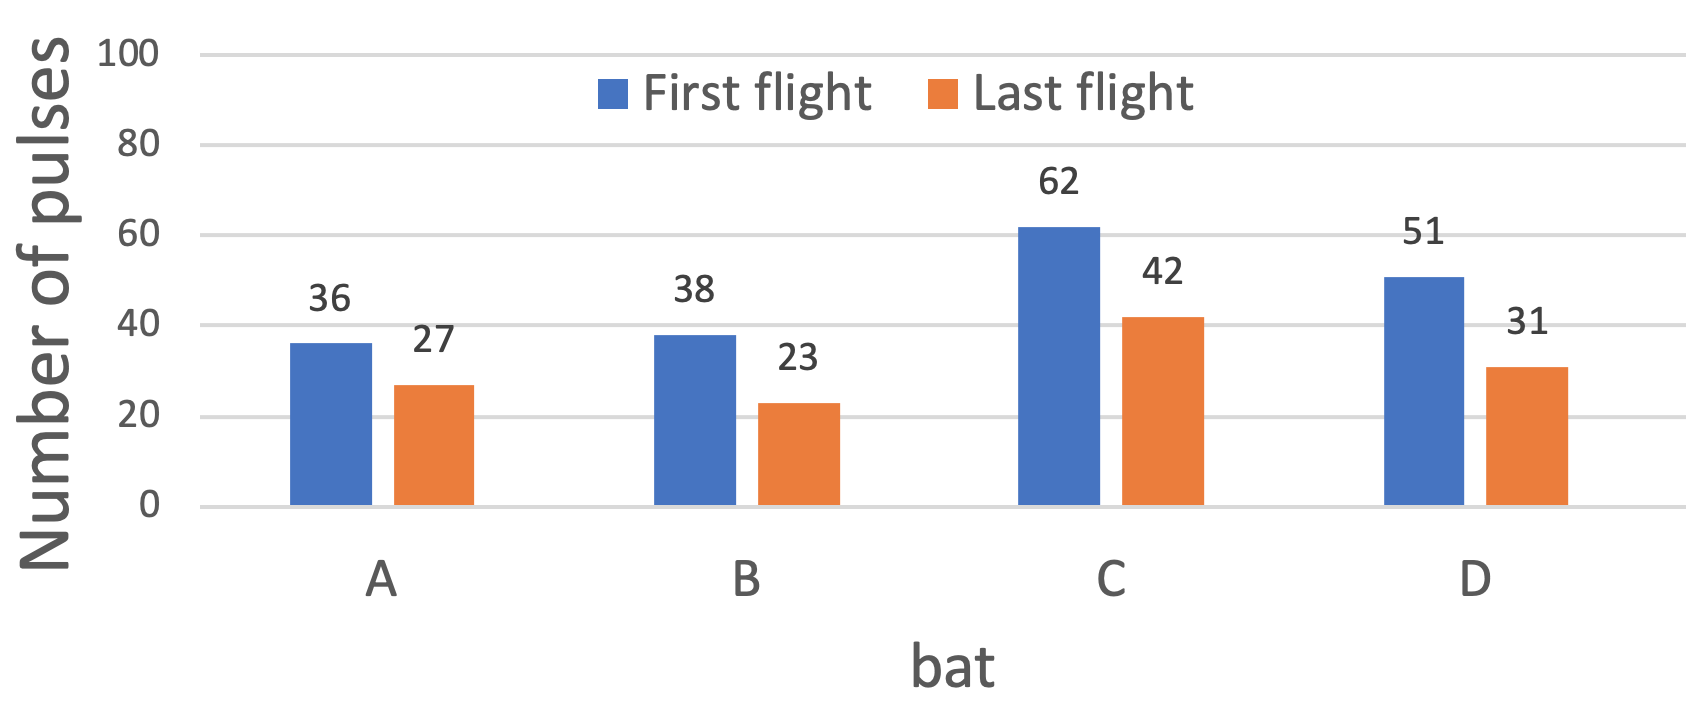
\includegraphics[width=13cm]{figures/bat_pulses.png}
  \caption{
    A decrease of the number of pulses at the first and last 
    flight of the bat.
  }\label{fig:bat_pulse}
\end{figure}
\vspace{\stretch{1}}


\newpage
\vspace*{\stretch{1}}
\begin{figure}[H]
  \centering
  \vfill
  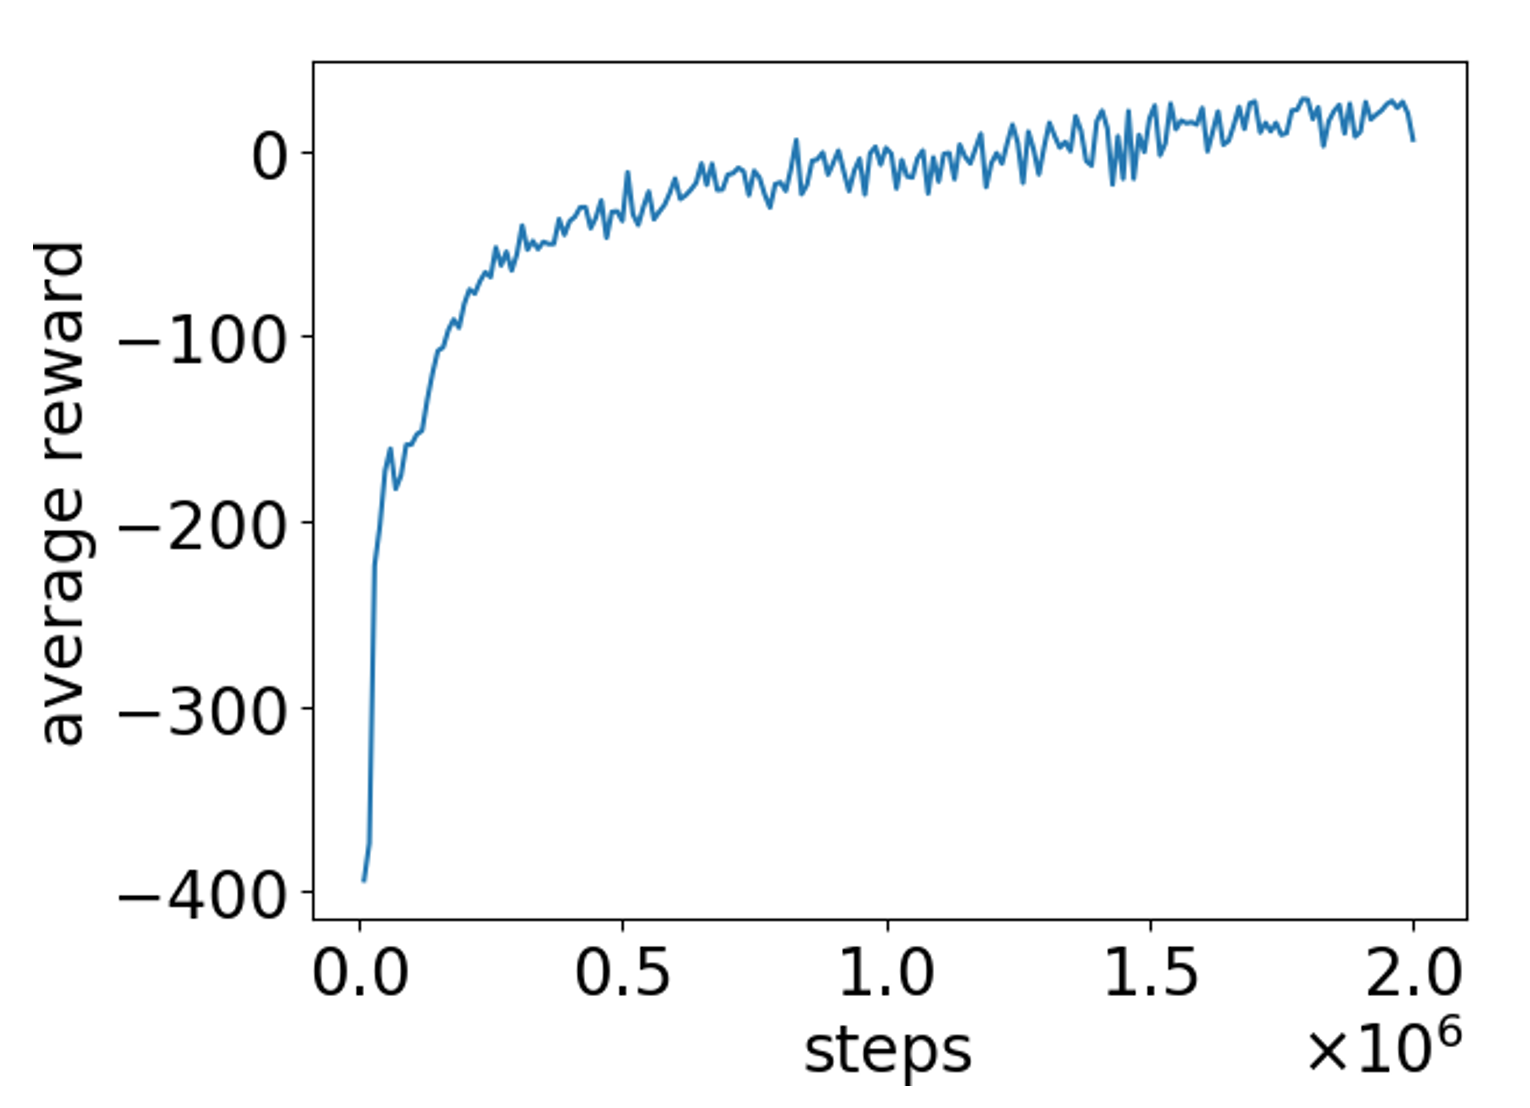
\includegraphics[width=10cm]{figures/training_development.png}
  \caption{
    Transition in average reward for every thousand steps.
    An increase of the average reward indicates that 
    the agent has learned better policy.
  }\label{fig:avearge_reward}
\end{figure}
\vspace{\stretch{1}}


\newpage
\vspace*{\stretch{1}}
\begin{figure}[H]
  \centering
  \vfill
  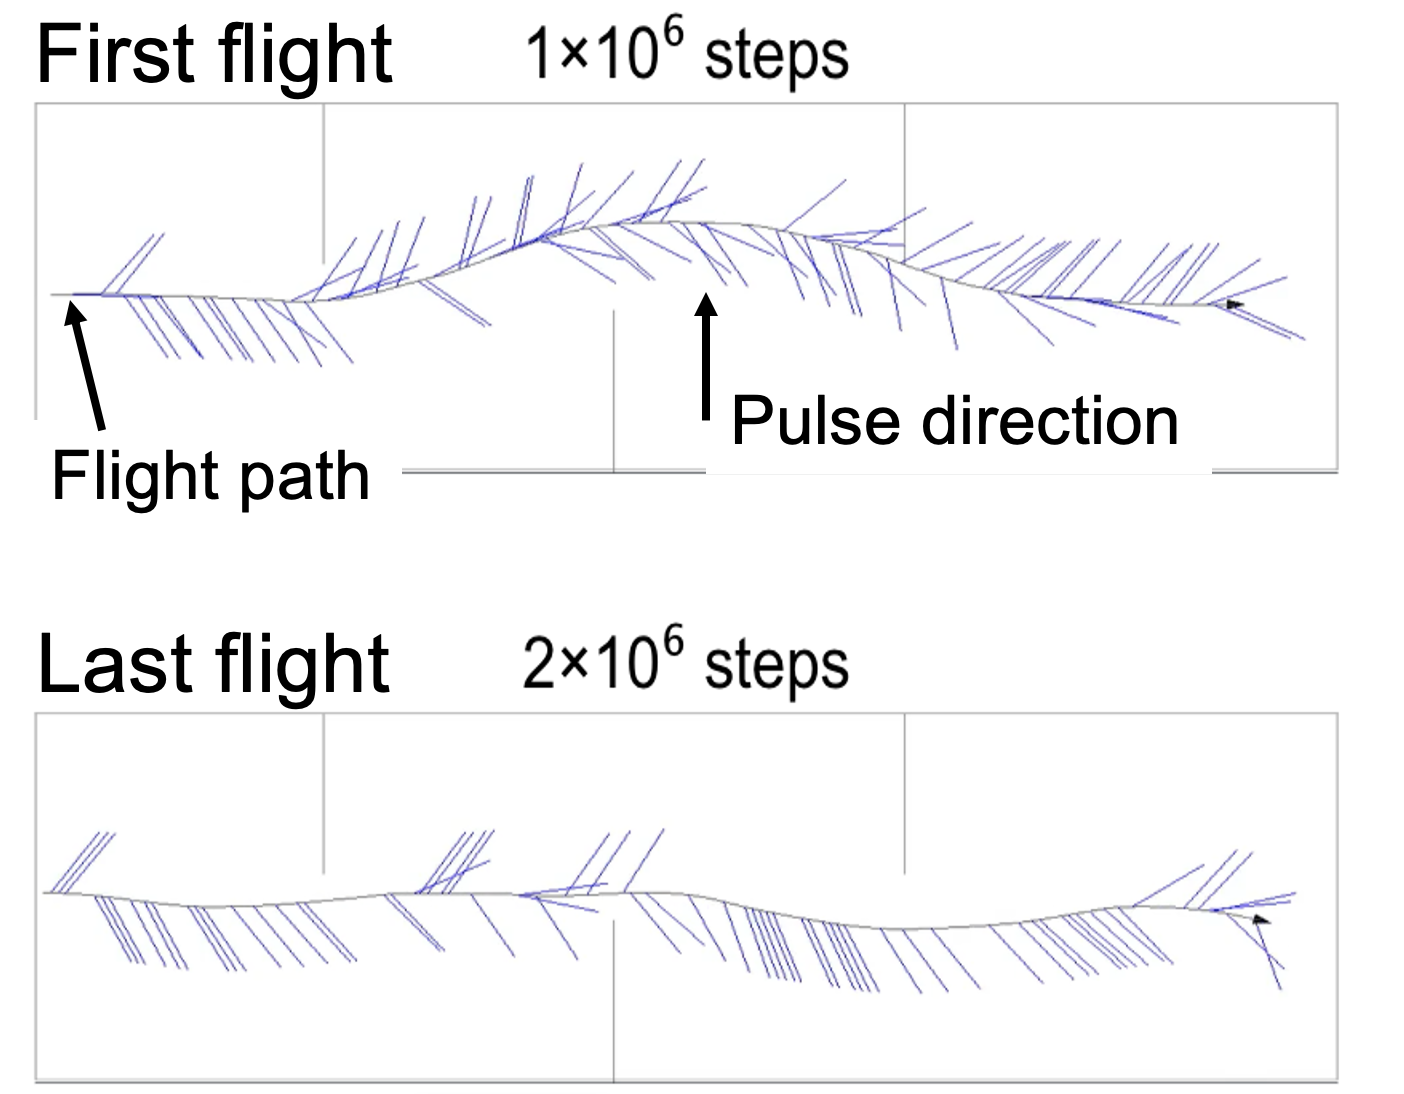
\includegraphics[width=12cm]{figures/agent_trajectory.png}
  \caption{
    Comparison between the first and last trajectory of the agent.
  }\label{fig:agent_trajectory}
\end{figure}
\vspace{\stretch{1}}


\newpage
\vspace*{\stretch{1}}
\begin{figure}[H]
  \centering
  \vfill
  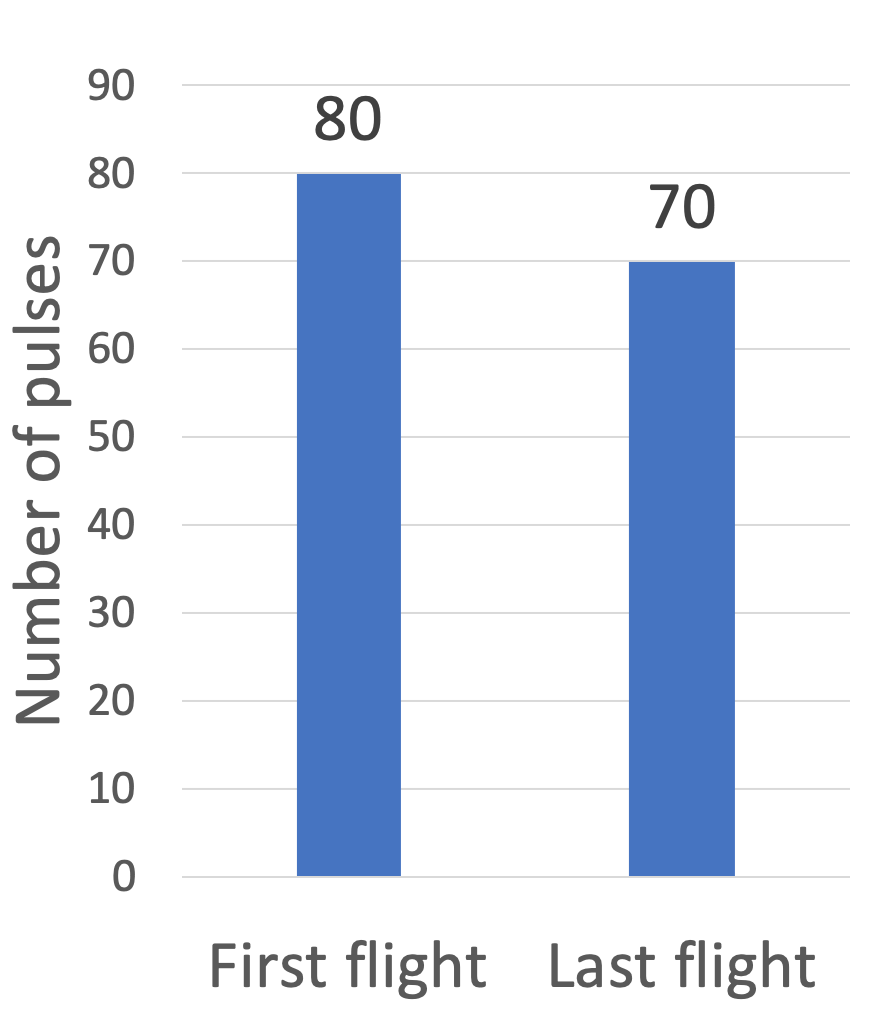
\includegraphics[width=7cm]{figures/agent_pulses.png}
  \caption{
    A decrease of the number of pulses 
    the first and last episode of the agent.
  }\label{fig:agent_pulse}
\end{figure}
\vspace{\stretch{1}}

\end{document}